% Source: Notion page “10. Web可视化与交互演示”. Generated without rewriting its content.
\chapter{Web可视化与交互演示}

\section{系统首页 / 总览页：}

\begin{figure}[htbp]
\centering
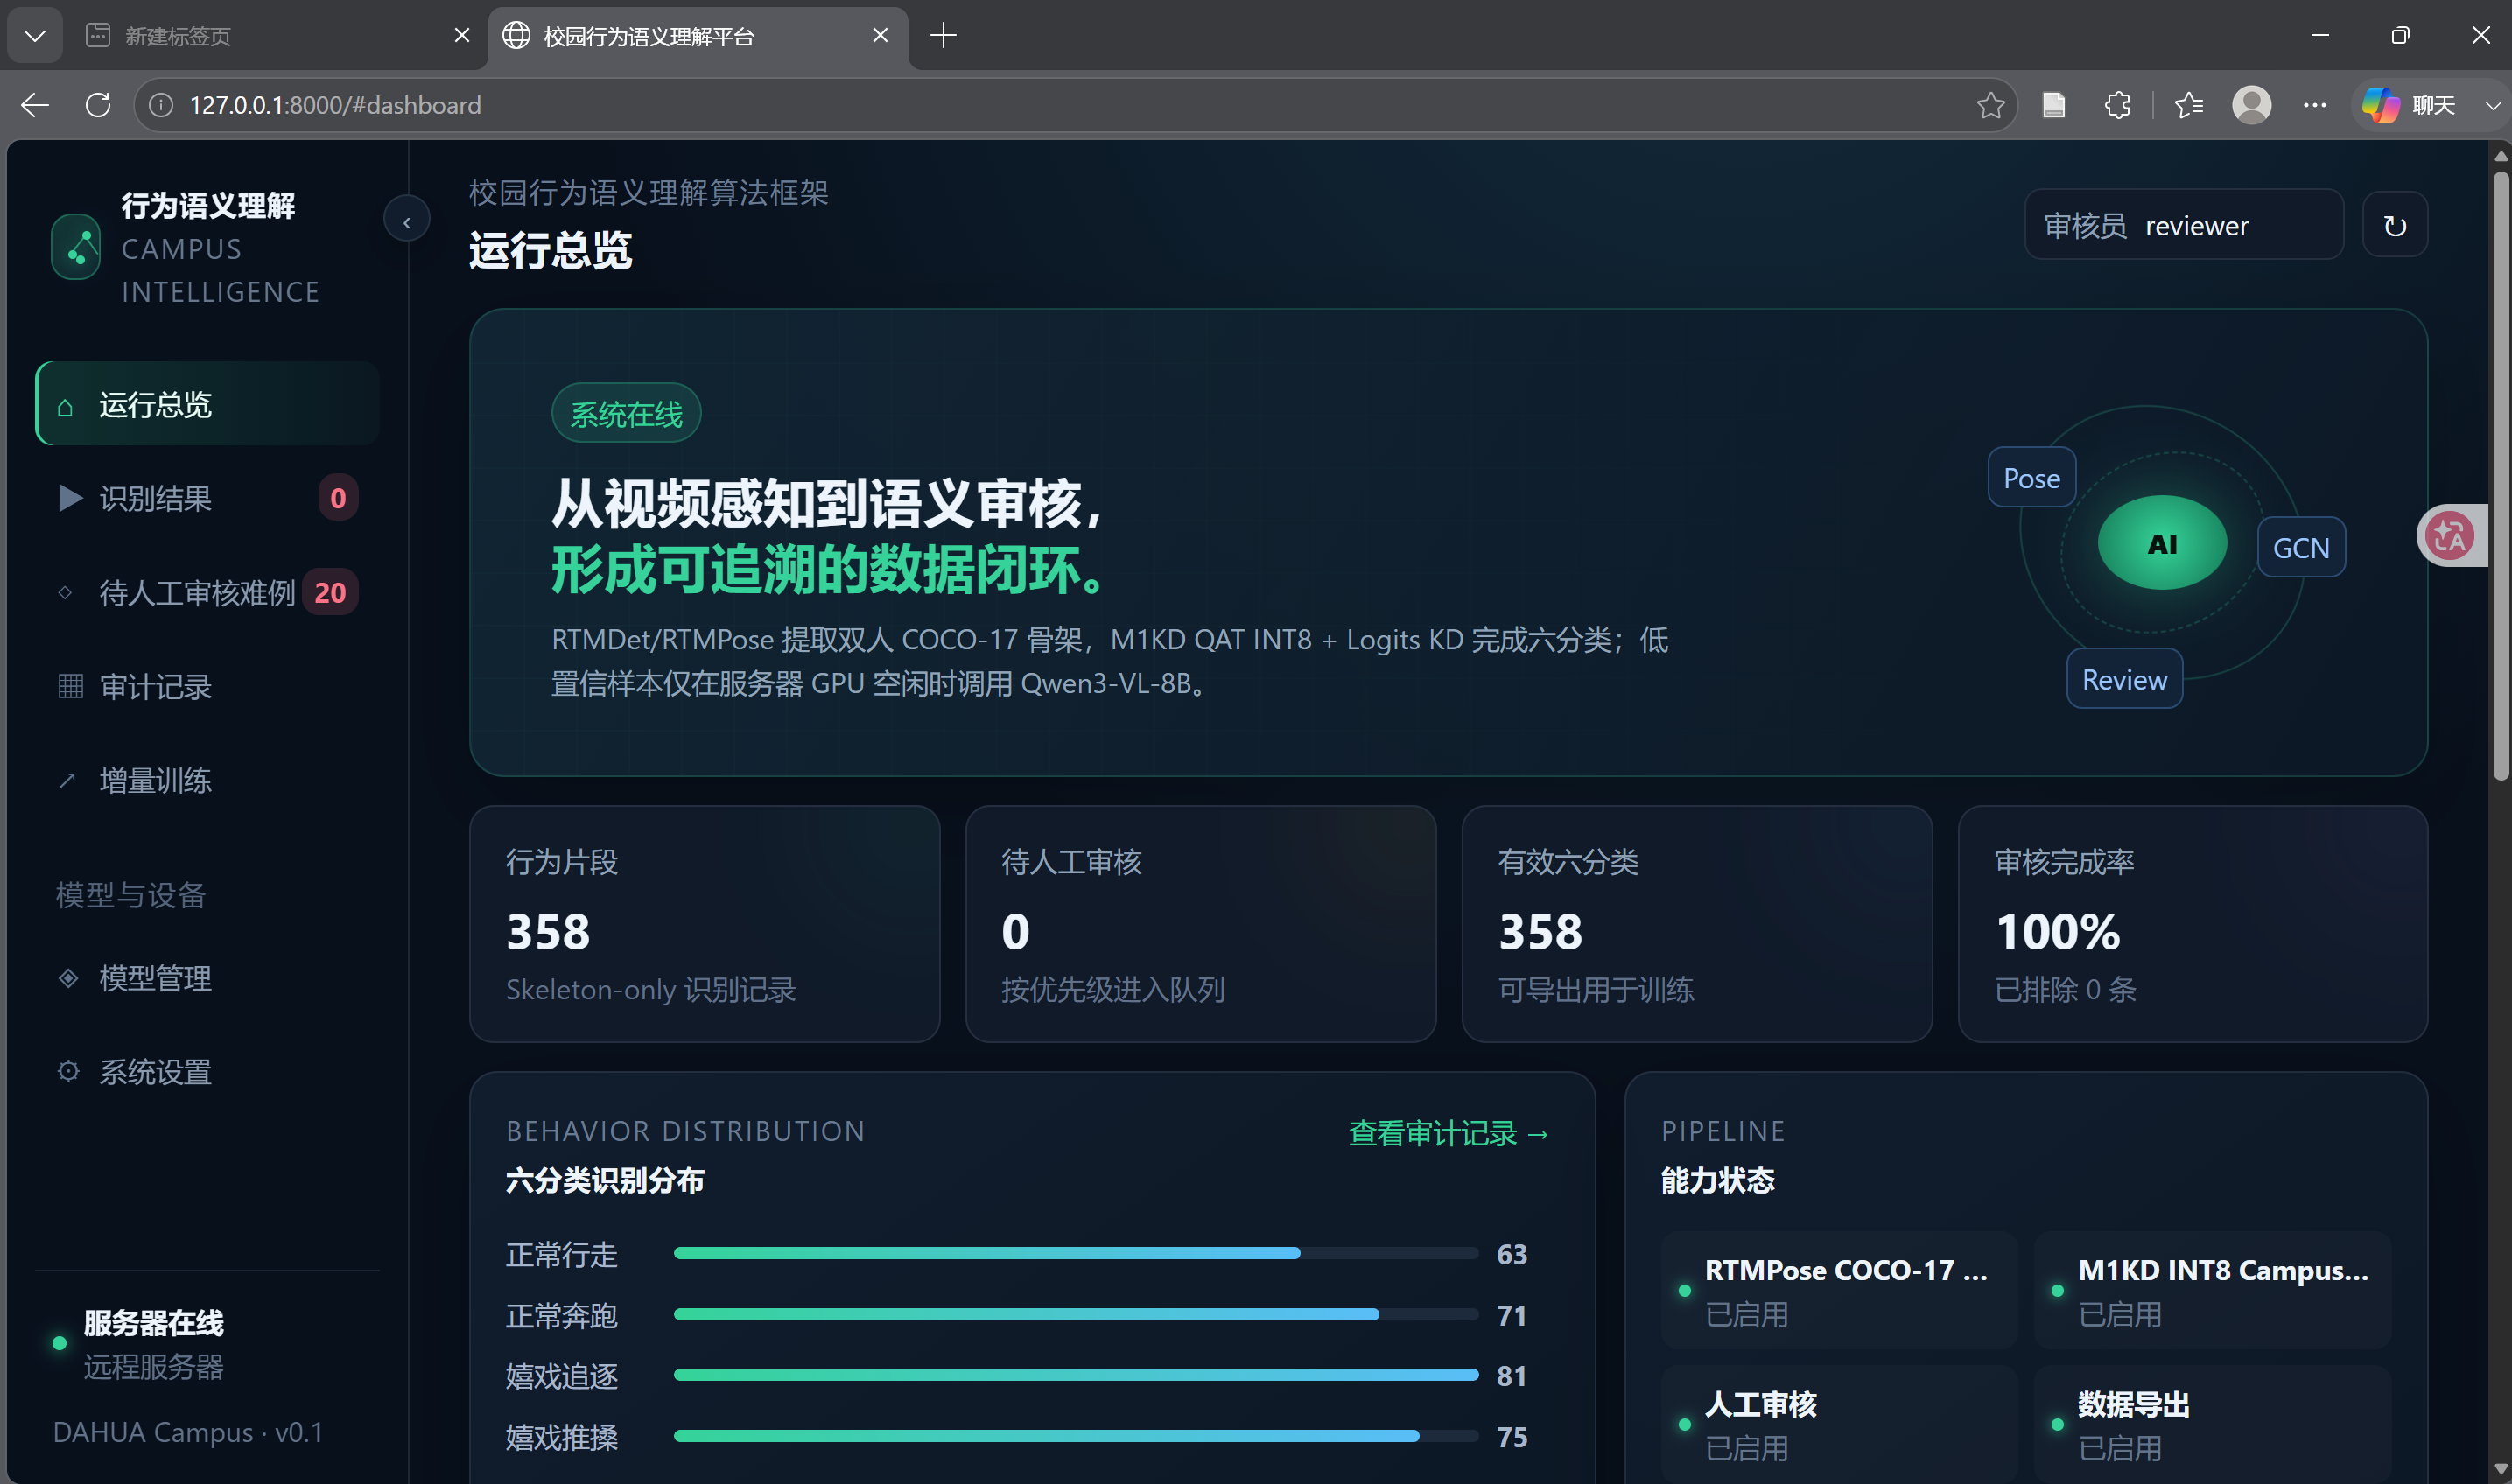
\includegraphics[width=0.96\linewidth,keepaspectratio]{figures/notion_image_07.png}
\end{figure}

\section{行为识别结果页：}

有样本选择栏、骨架流视频、六分类Logits、人工标注栏、大模型分析（如果同时是“待人工审核难例”

\begin{figure}[htbp]
\centering
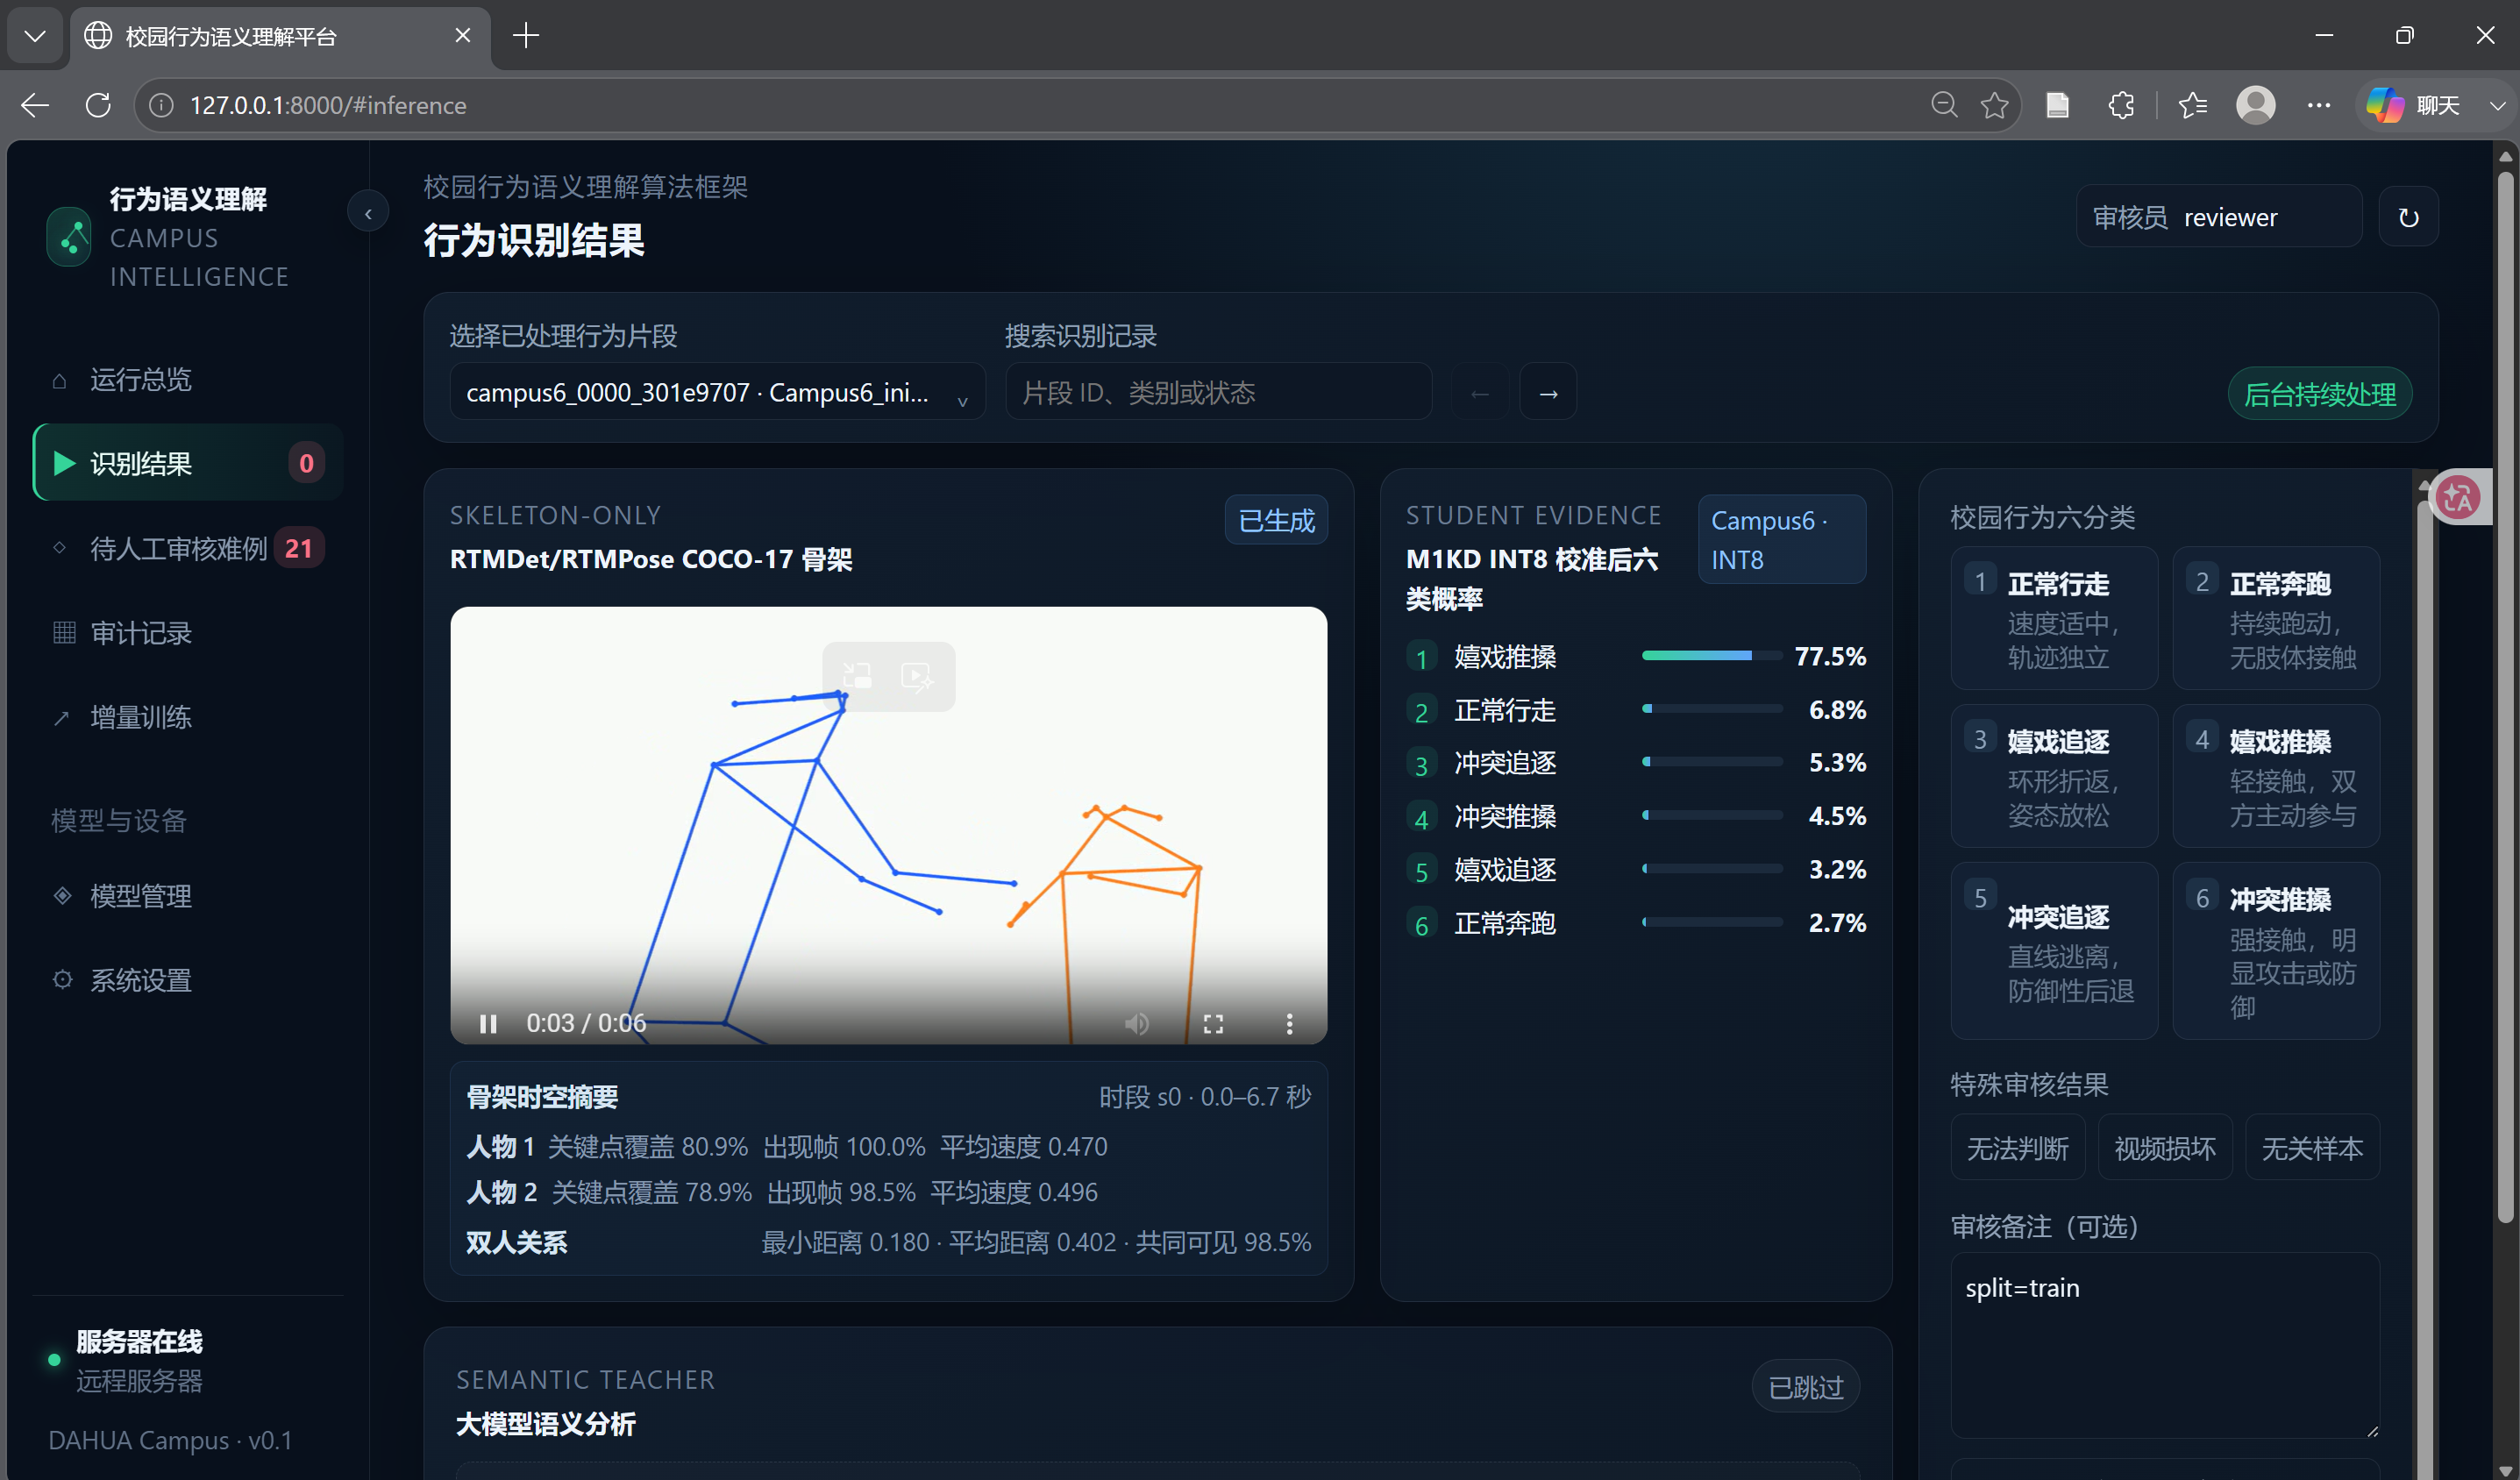
\includegraphics[width=0.96\linewidth,keepaspectratio]{figures/notion_image_08.png}
\end{figure}

\section{大模型伪标签和人工审核页}

\begin{figure}[htbp]
\centering
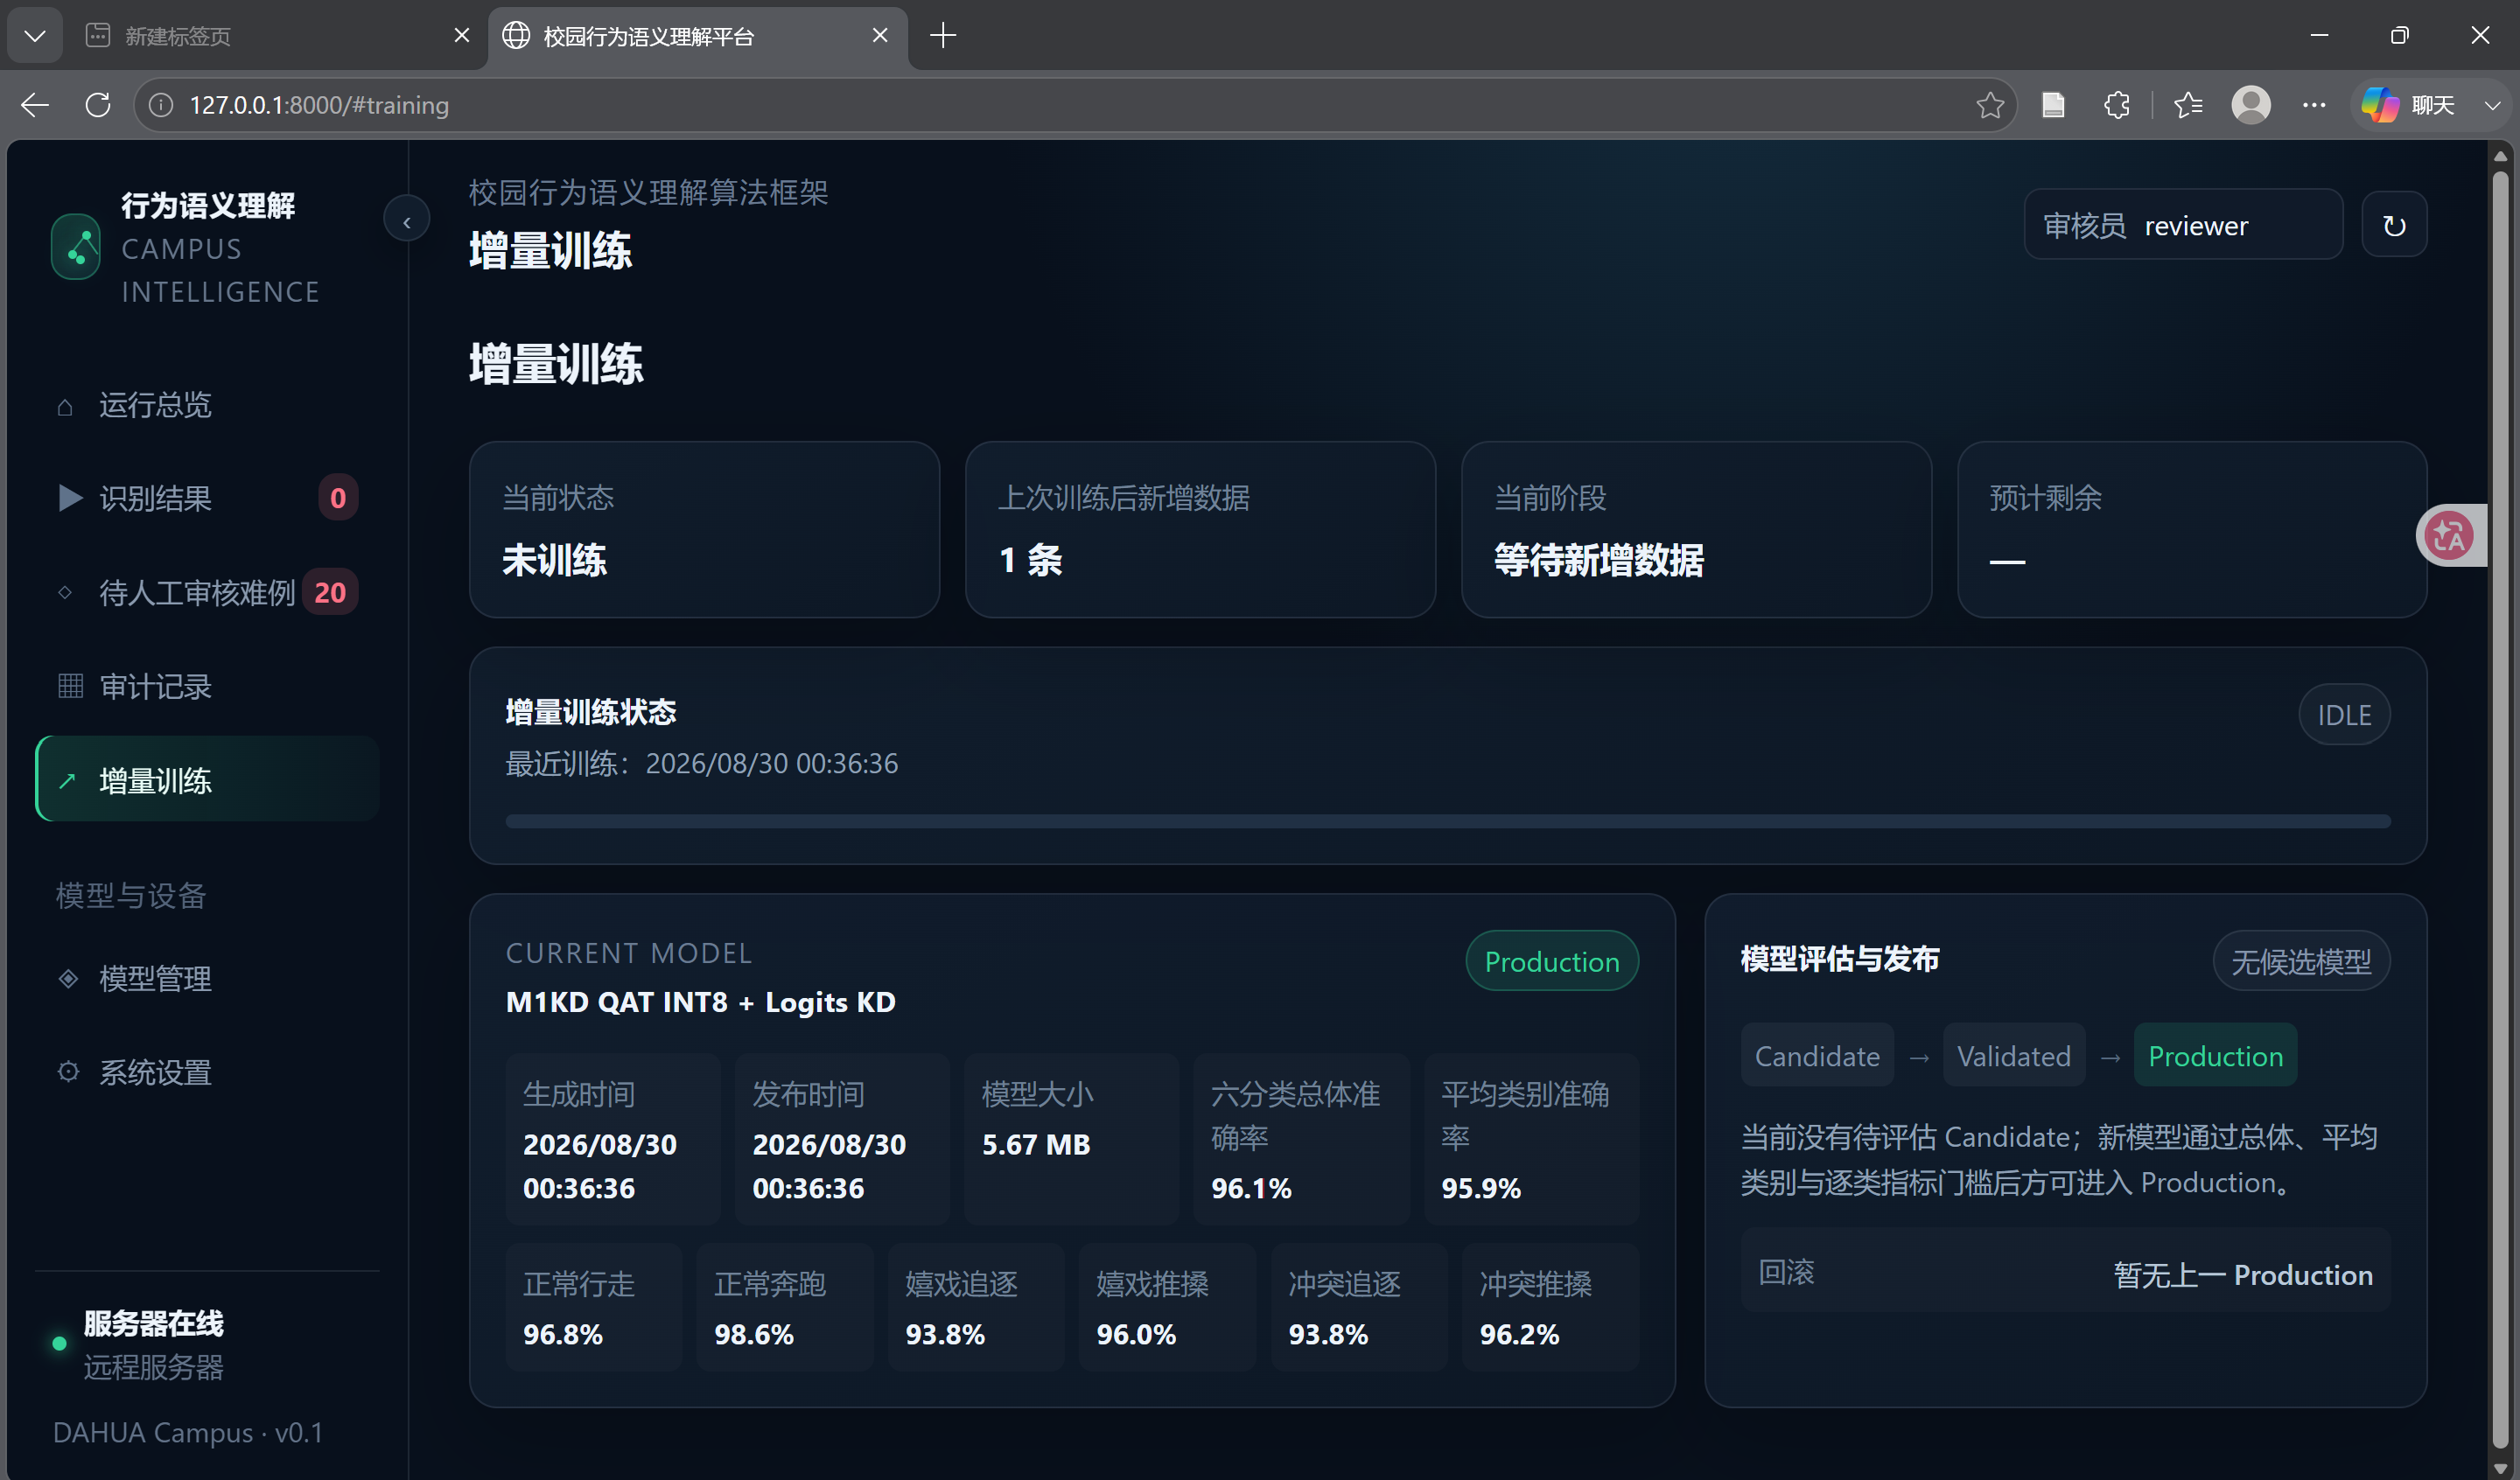
\includegraphics[width=0.96\linewidth,keepaspectratio]{figures/notion_image_09.png}
\end{figure}

\section{增量学习和模型迭代页}

\section{模型管理页}

\begin{figure}[htbp]
\centering
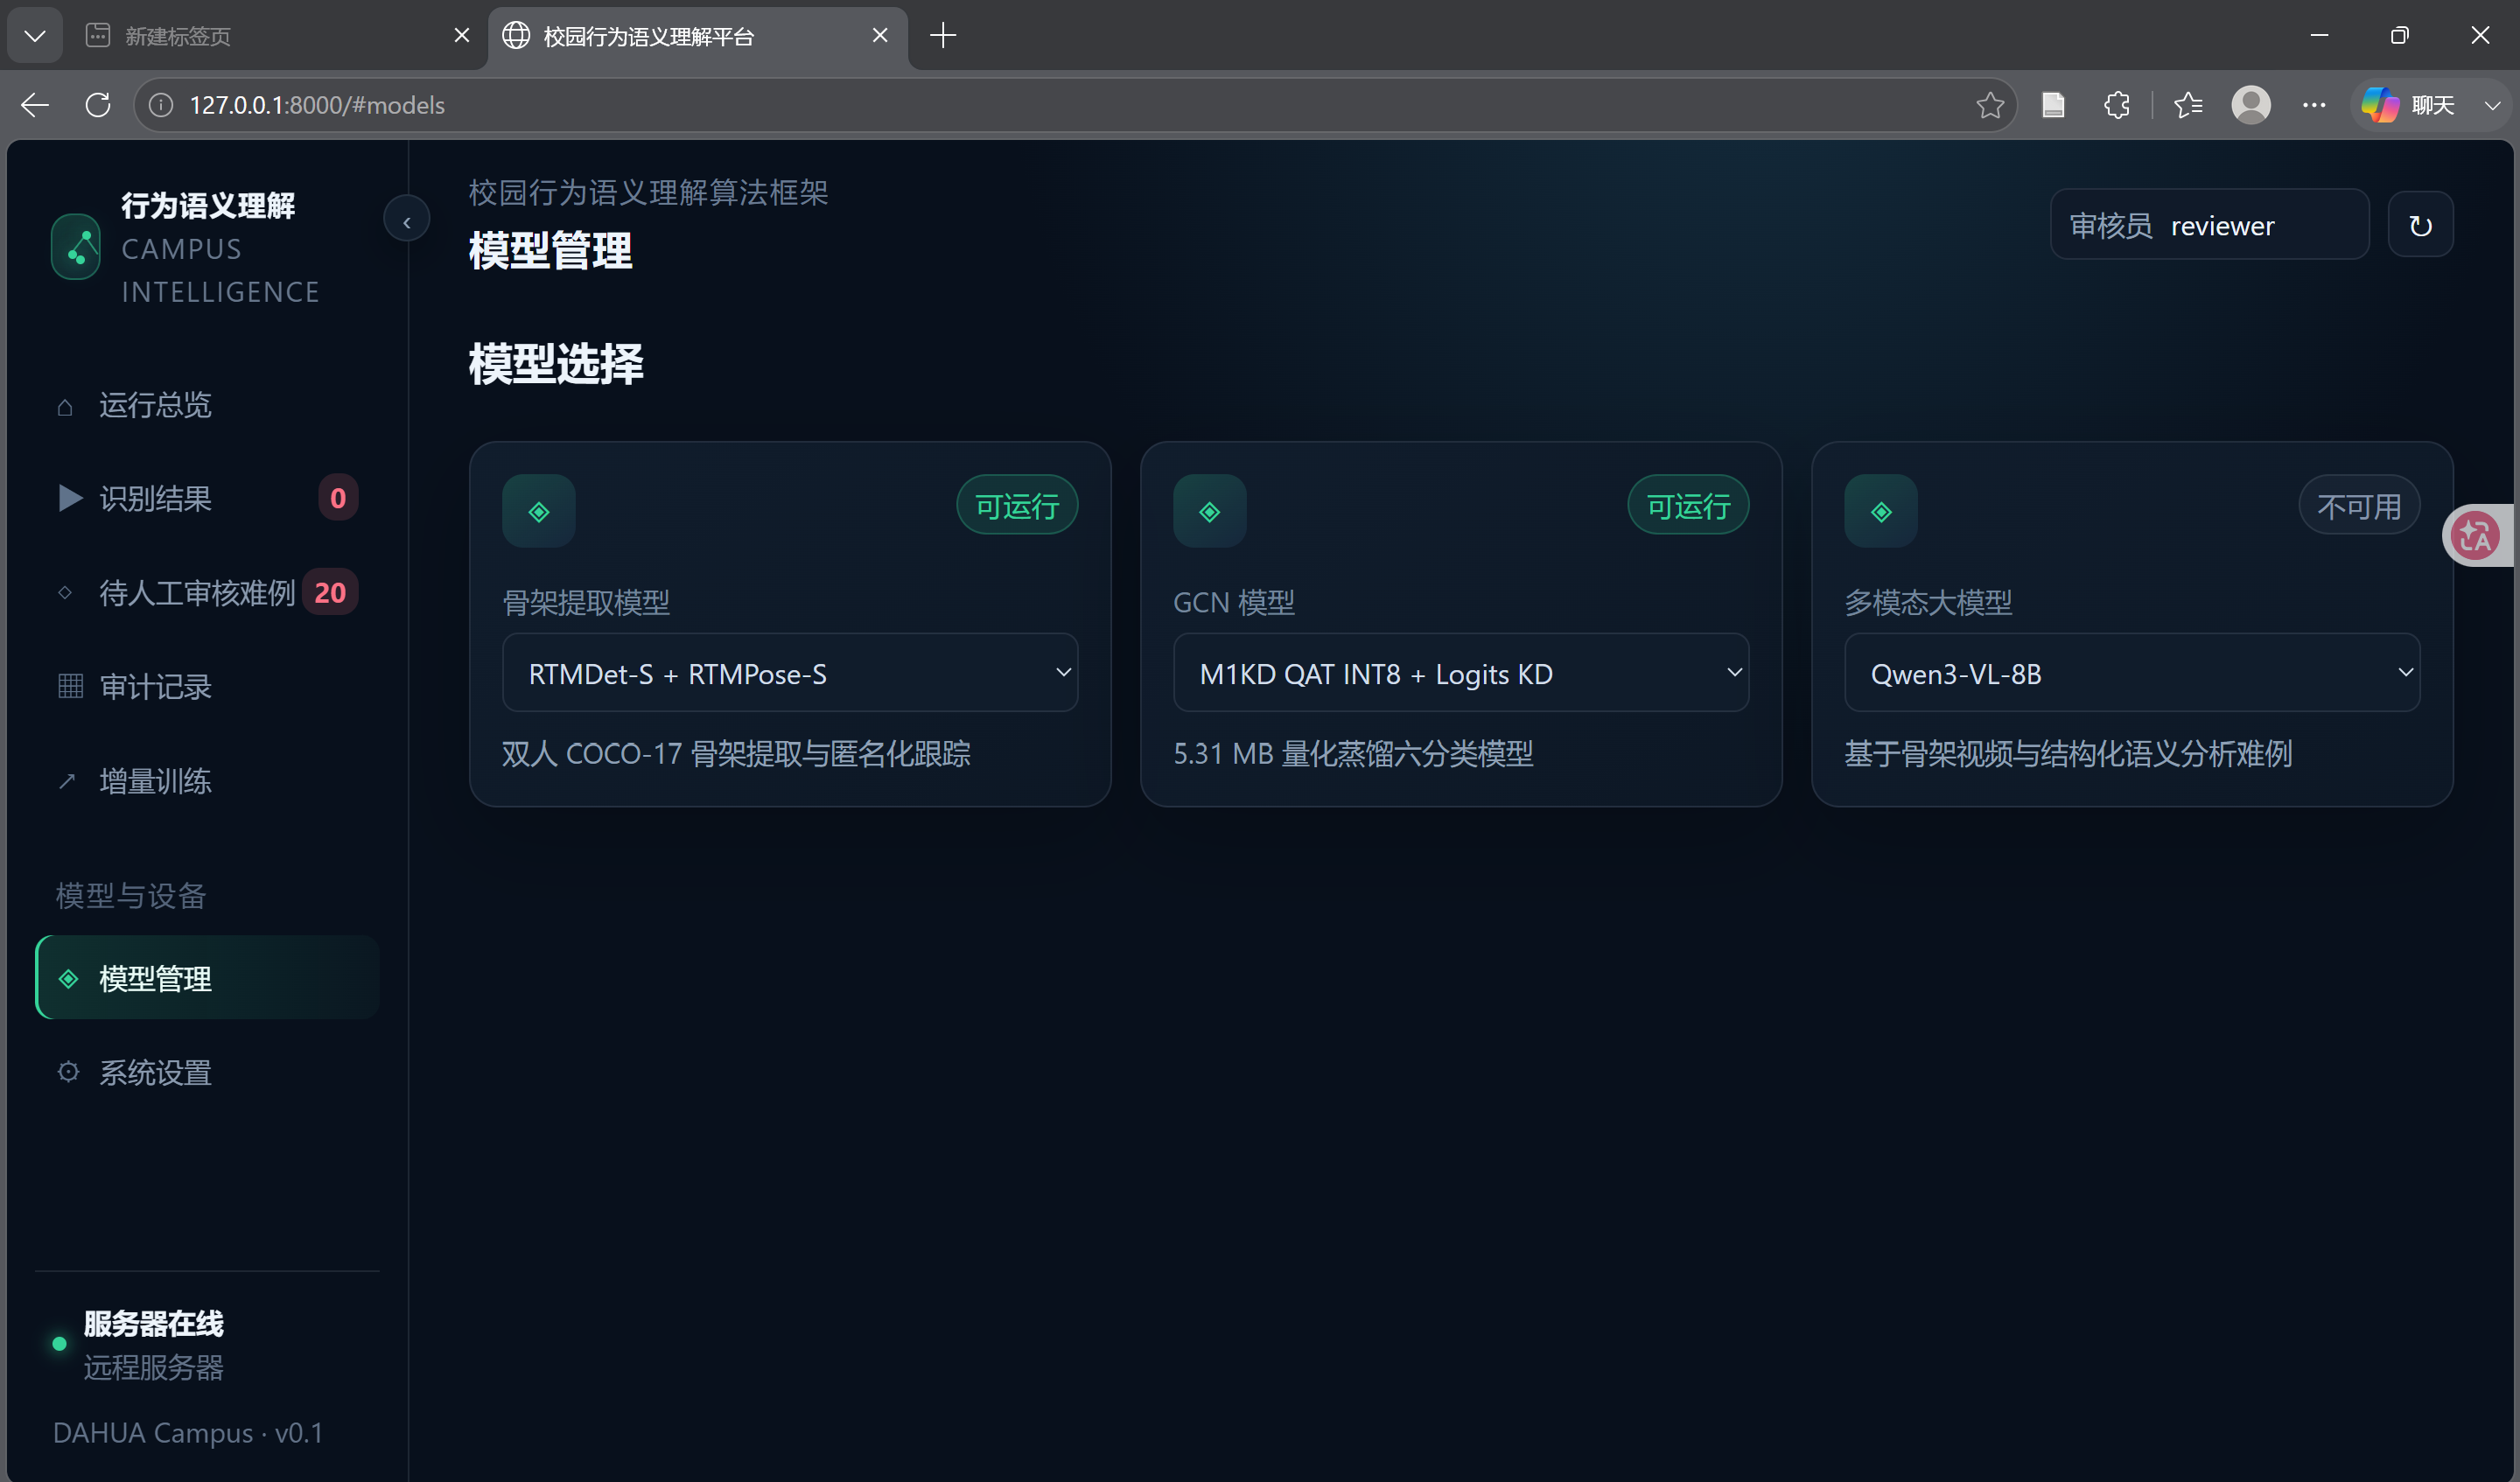
\includegraphics[width=0.96\linewidth,keepaspectratio]{figures/notion_image_10.png}
\end{figure}

\section{系统设置页}

\begin{figure}[htbp]
\centering
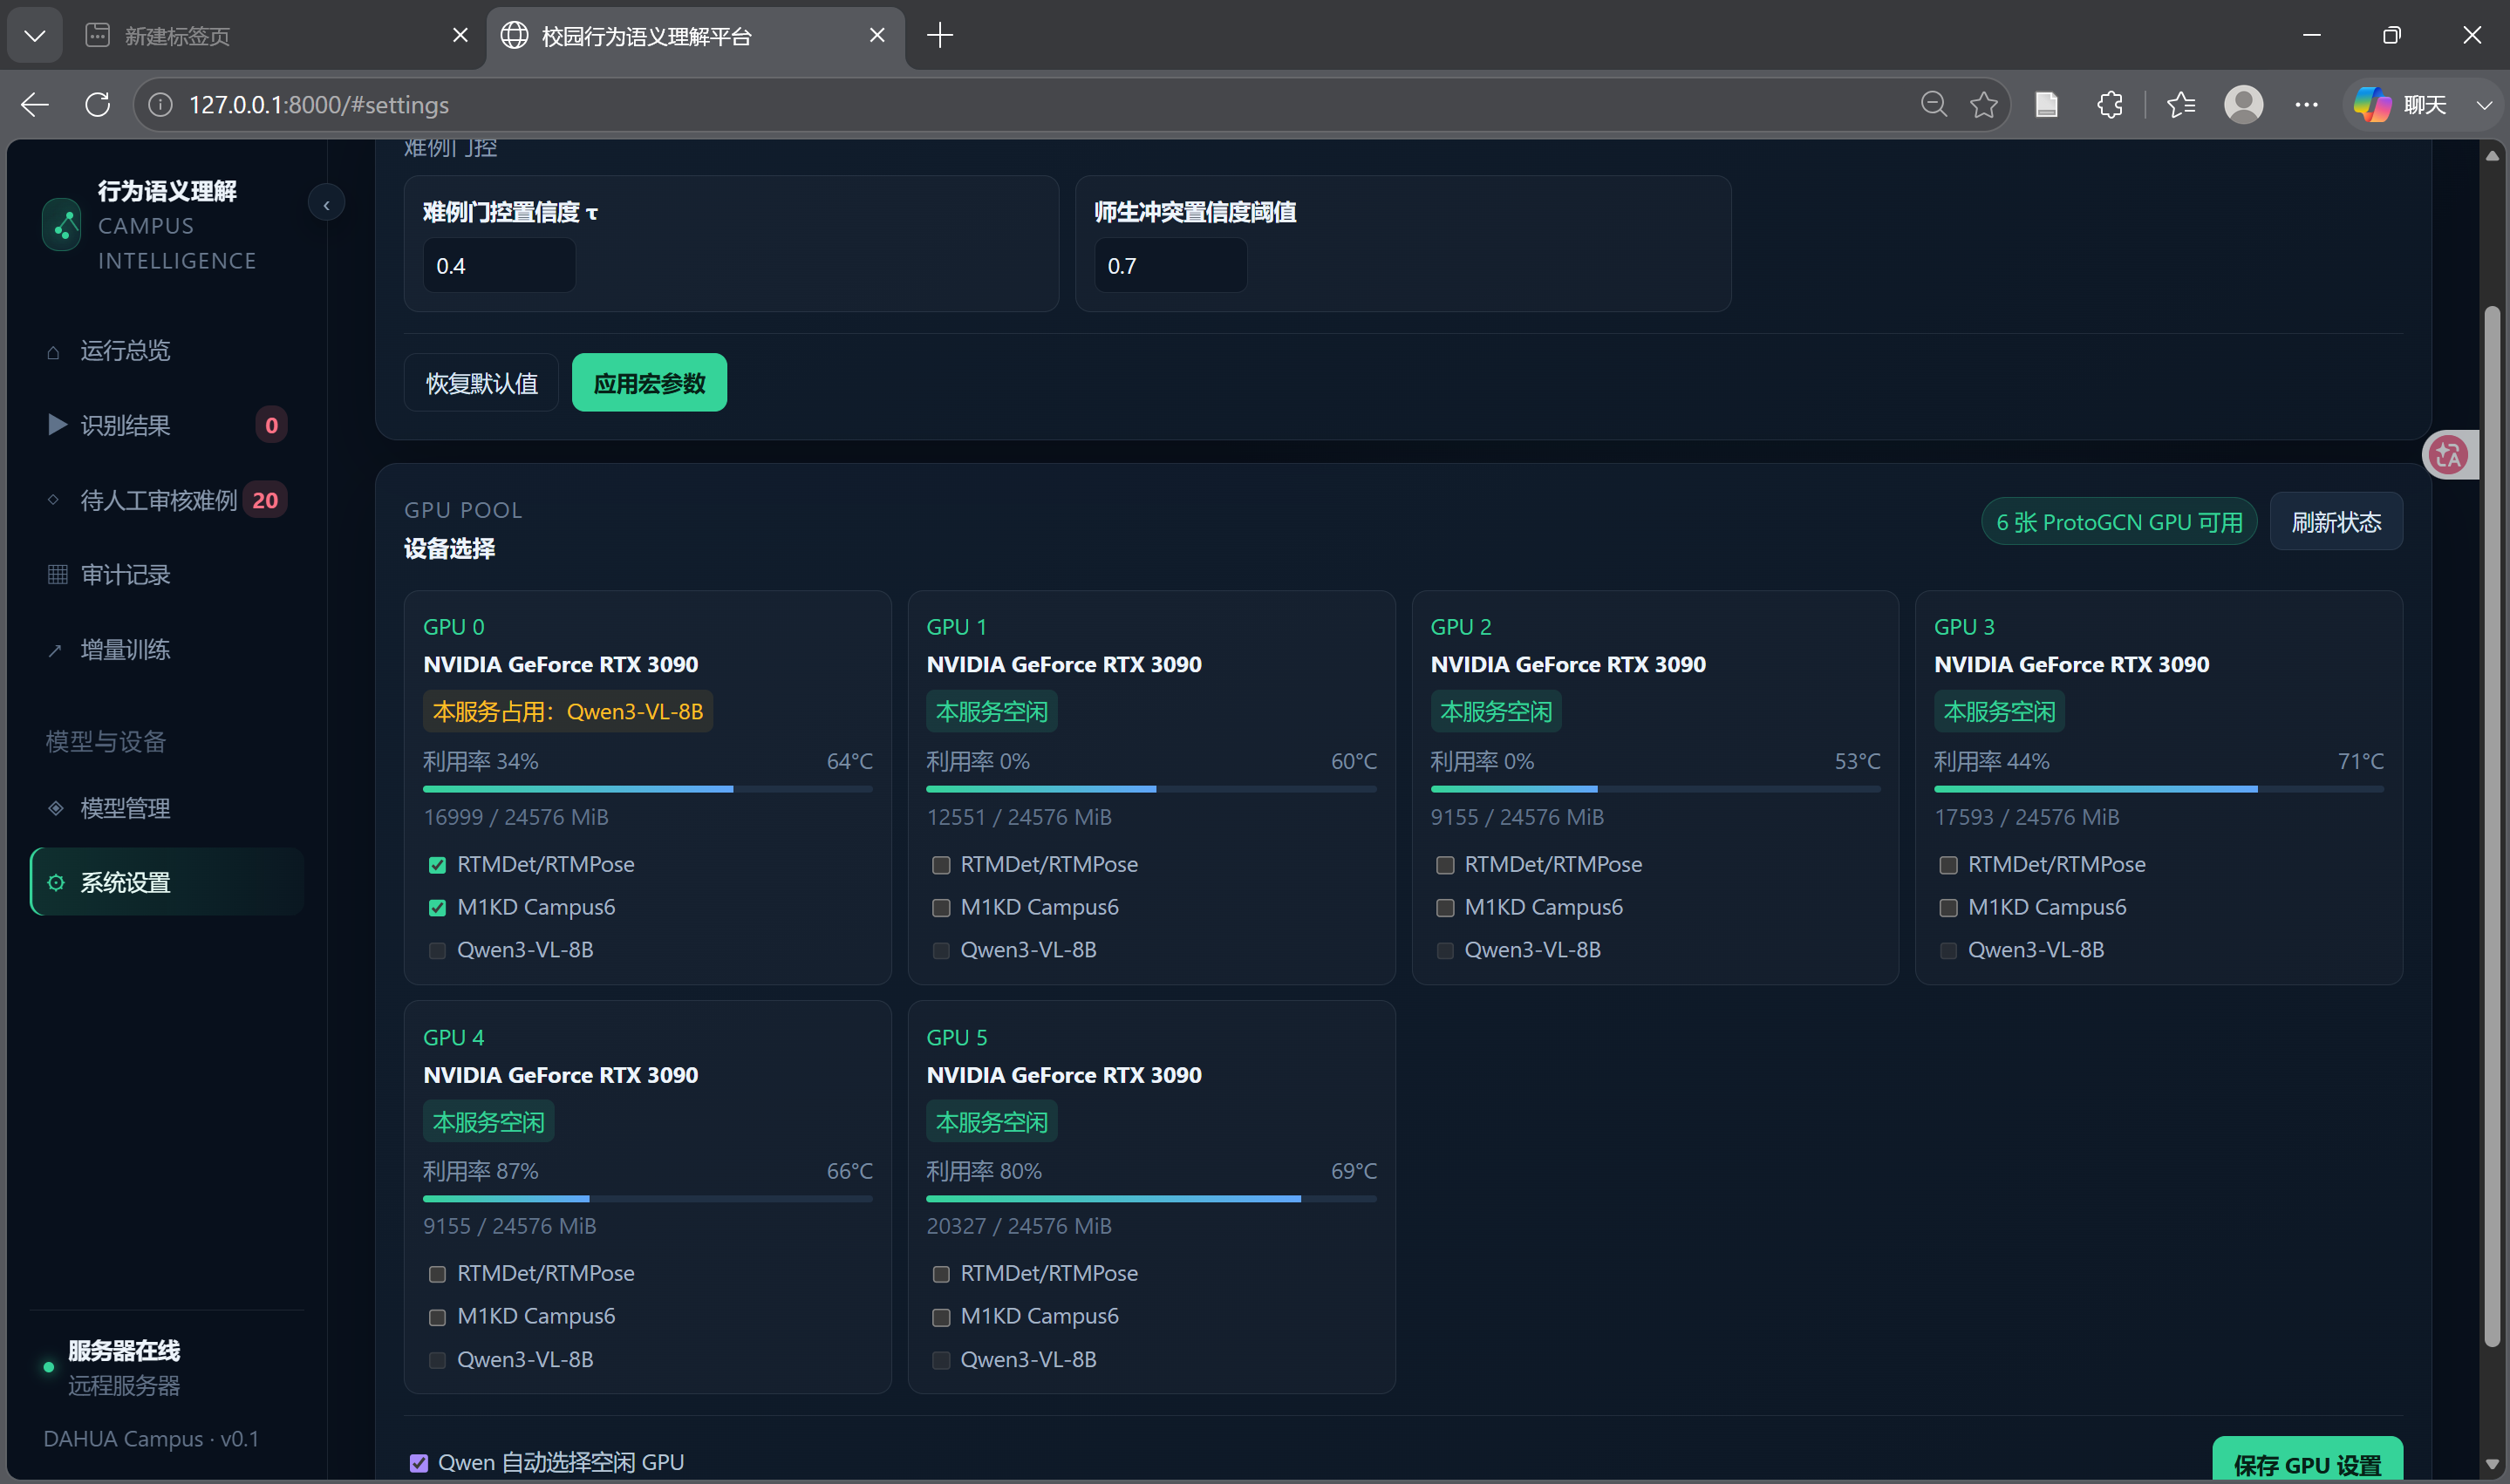
\includegraphics[width=0.96\linewidth,keepaspectratio]{figures/notion_image_11.png}
\end{figure}

